\documentclass{beamer}
\input{../../packages.tex}
\input{../../slides_formatting.tex}

% Remove drop shadow by title
% https://tex.stackexchange.com/questions/3139/beamer-how-to-remove-shadow-under-the-title-on-a-given-frame
\setbeamertemplate{title page}[default][colsep=-4bp,rounded=true]

%gets rid of footer
%will override 'frame number' instruction above
%comment out to revert to previous/default definitions
\setbeamertemplate{footline}{}

%gets rid of bottom navigation symbols
\setbeamertemplate{navigation symbols}{}


\setbeamerfont*{frametitle}{family=\rmfamily, parent=structure}

%Information to be included in the title page:
\title{UFL + FEniCS: DSL Case Study}
\author{Russell Bentley}
\institute{
  Stony Brook University
}

\date{September 18 2025}

\begin{document}
\fontfamily{cmr}\selectfont

%\placelogofalse
\begin{frame}{SALTAR DSL}
\begin{center}
\centering
%\shadowimage[width=2.5cm]{example_1.png}

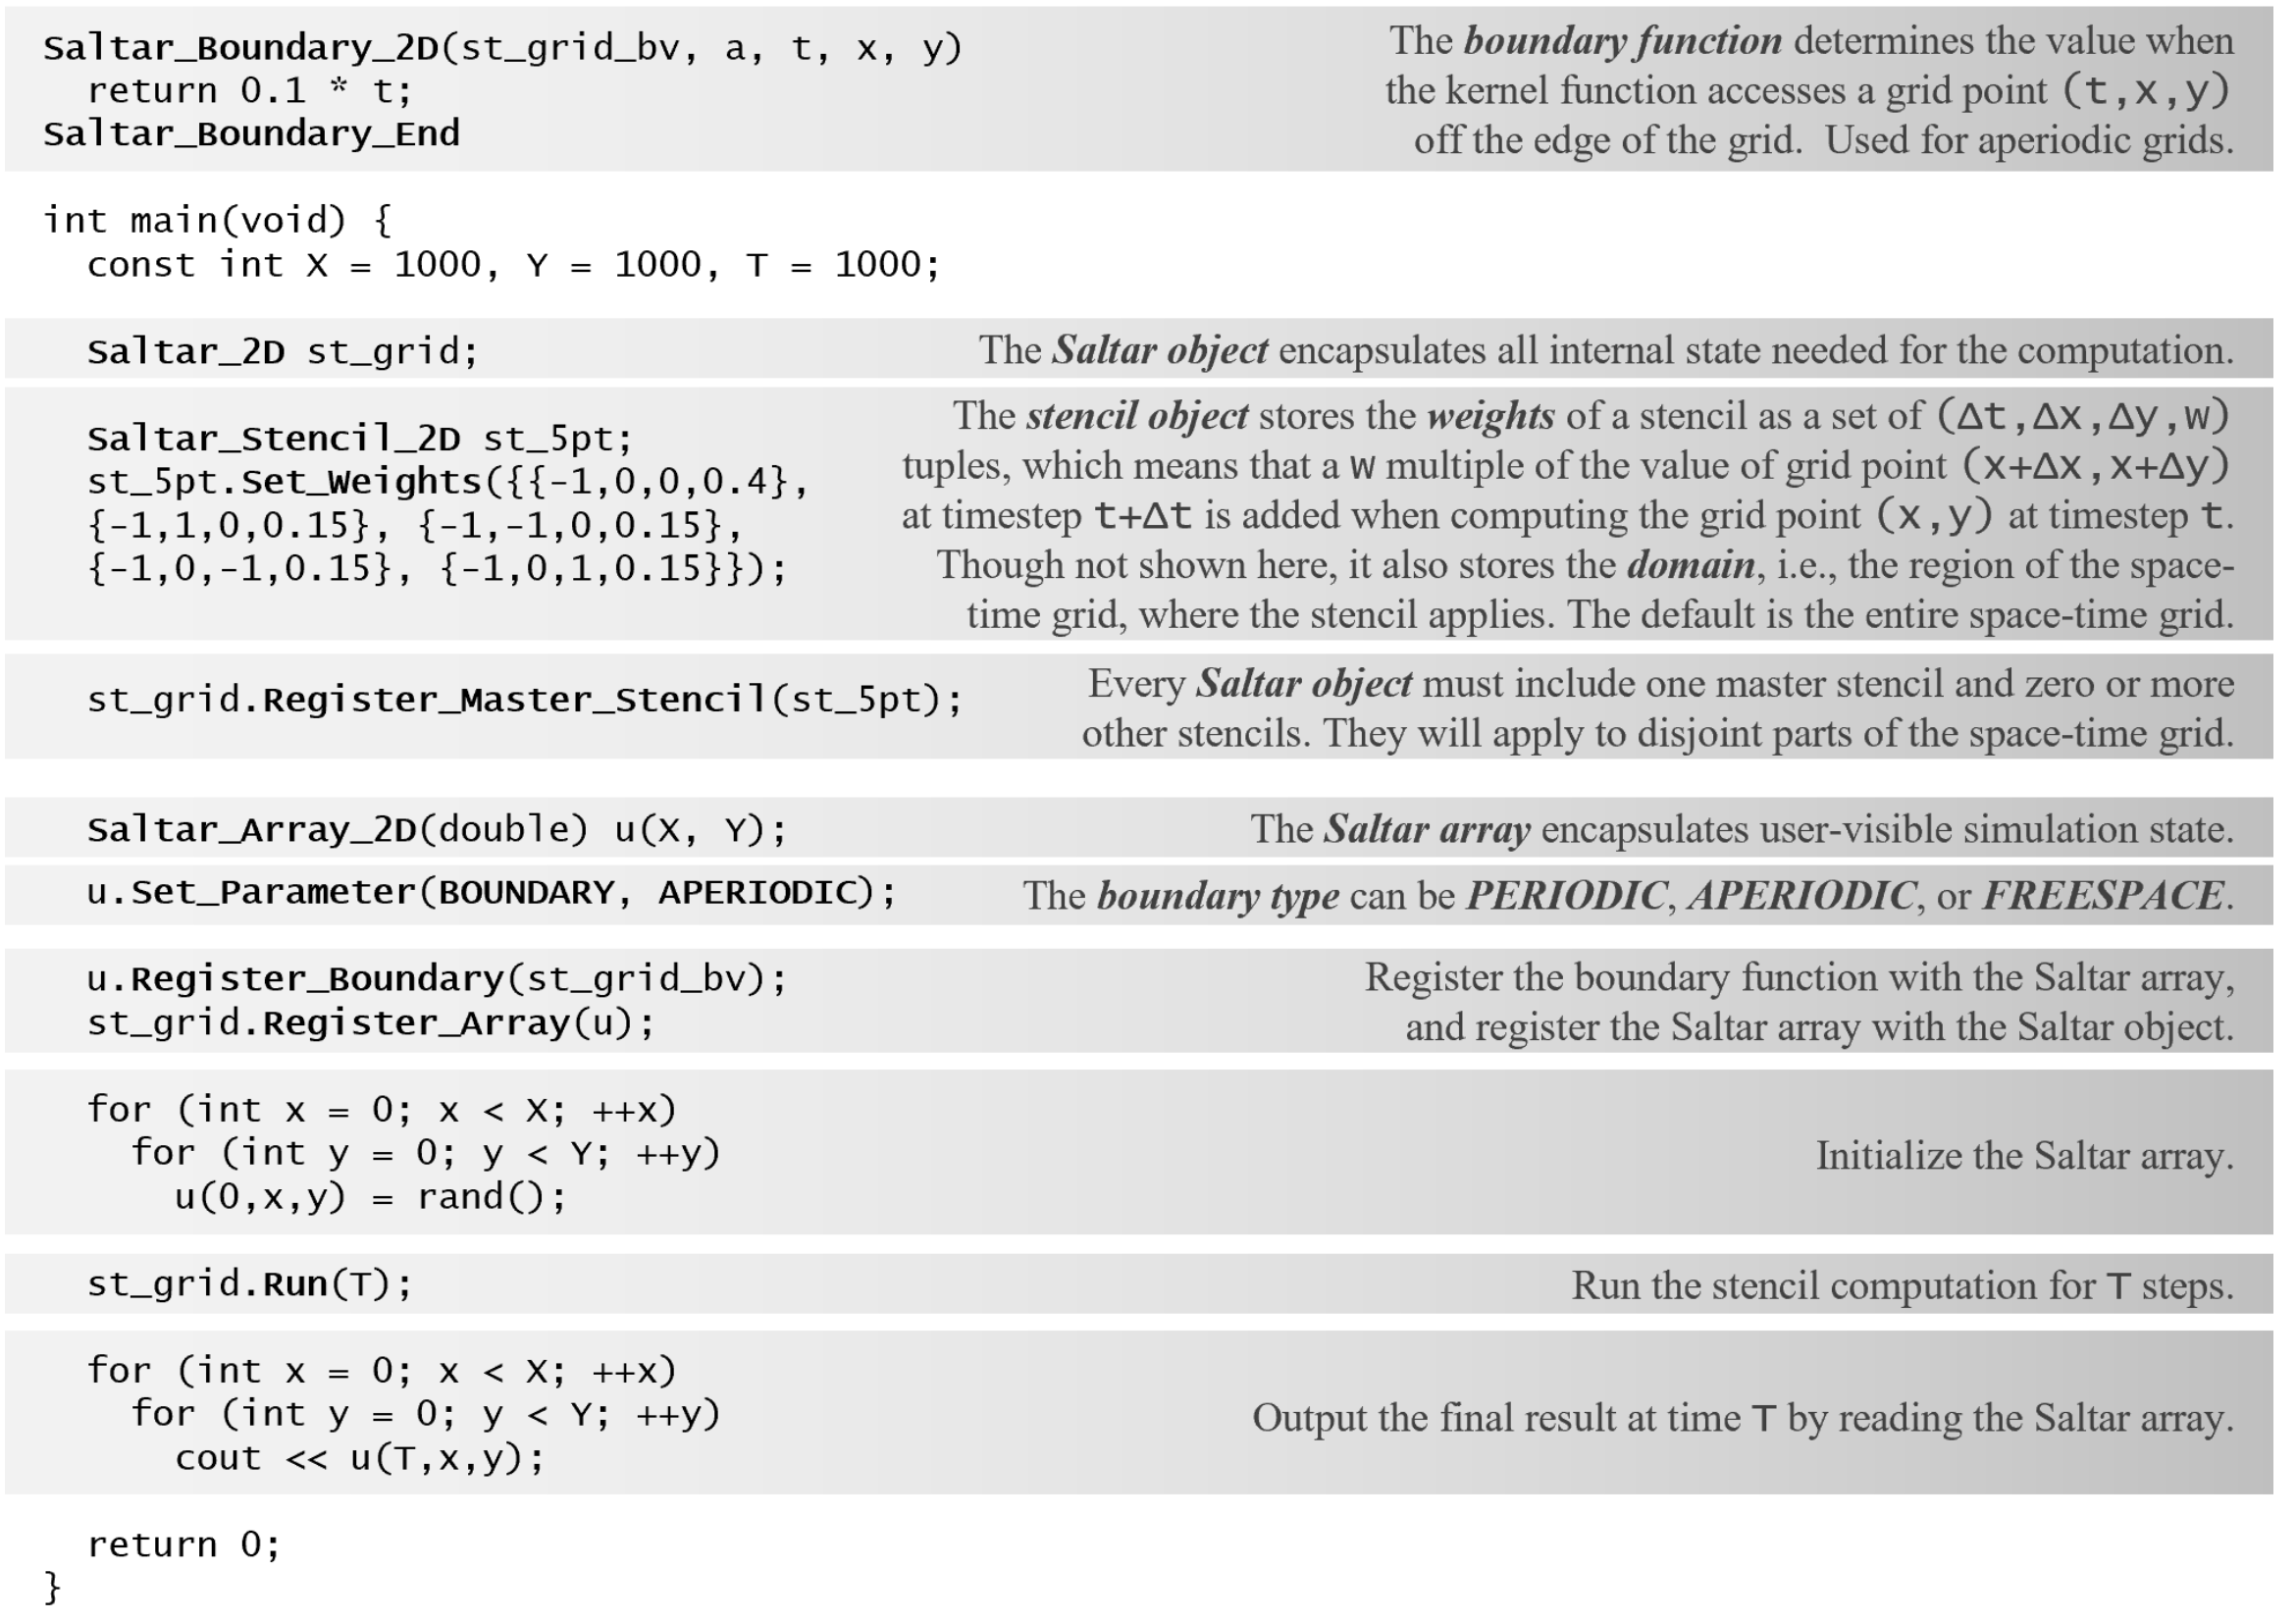
\includegraphics[width=8cm]{saltar_prop.png}

% [trim={left bottom right top},clip]
%
\includegraphics[width=8.5cm, page=3, trim={0 9cm 14cm 0cm},clip]{assets/vec_db_figs.pdf}
\end{center}
\end{frame}
%\placelogotrue

%\placelogofalse
\begin{frame}{DSEL in Python}
\begin{columns}
\column{0.58\linewidth}
\centering
\begin{outline}
  \1 SALTAR Programs
  \2 Declarative
  \2 Symbolic
  \1 Great fit for SymPy based IR
  \1 Follow other numerical methods
  \2 \lstinline{lbmpy}
  \2 FEniCS + UFL
\end{outline}

\column{0.38\linewidth}
\begin{center}
\centering
%\shadowimage[width=2.5cm]{example_1.png}


\includegraphics[width=2.5cm]{fenics_logo.png}

\vspace{0.2cm}



\includegraphics[width=2.5cm]{logo-3.png}

% [trim={left bottom right top},clip]
%
\includegraphics[width=8.5cm, page=3, trim={0 9cm 14cm 0cm},clip]{assets/vec_db_figs.pdf}
\end{center}
\end{columns}
\end{frame}
%\placelogotrue
\end{document}


